% Partial composition of trees: T o_2 S grafts the root of S onto the second leaf of T.
\documentclass[border=2pt]{standalone}
\usepackage{tikz}
% Shared colours of the research figures (matplotlib tab10, as in the Berkovich skeleton figure).
\usepackage{amsmath}
\usetikzlibrary{calc}
\definecolor{figink}{HTML}{262626}
\definecolor{figred}{HTML}{D62728}
\definecolor{figblue}{HTML}{1F77B4}

\begin{document}
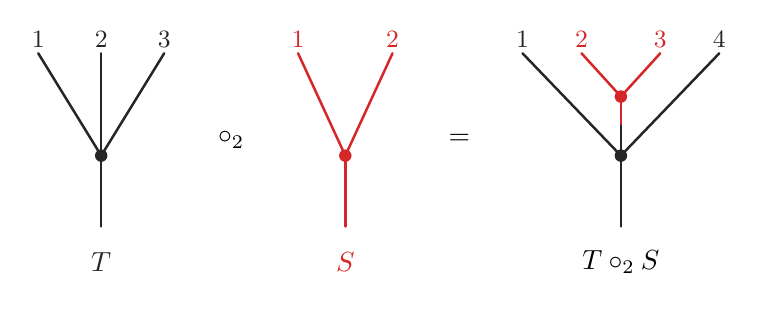
\begin{tikzpicture}[
    scale=1.0,
    edge/.style={line width=0.9pt, line cap=round},
    vtx/.style={circle, fill, inner sep=0pt, minimum size=4.5pt},
    leaf/.style={font=\small, anchor=south, inner sep=1.5pt},
  ]
  % T: a corolla with three leaves
  \begin{scope}[figink]
    \draw[edge] (0,0) -- (0,0.9);
    \foreach \x/\l in {-0.8/1, 0/2, 0.8/3}
      \draw[edge] (0,0.9) -- (\x,2.2) node[leaf] {$\l$};
    \node[vtx] at (0,0.9) {};
    \node at (0,-0.45) {$T$};
  \end{scope}

  \node at (1.65,1.1) {$\circ_2$};

  % S: a corolla with two leaves
  \begin{scope}[xshift=3.1cm, figred]
    \draw[edge] (0,0) -- (0,0.9);
    \foreach \x/\l in {-0.6/1, 0.6/2}
      \draw[edge] (0,0.9) -- (\x,2.2) node[leaf] {$\l$};
    \node[vtx] at (0,0.9) {};
    \node at (0,-0.45) {$S$};
  \end{scope}

  \node at (4.55,1.1) {$=$};

  % T o_2 S
  \begin{scope}[xshift=6.6cm]
    \draw[edge, figink] (0,0) -- (0,0.9);
    \draw[edge, figink] (0,0.9) -- (-1.25,2.2) node[leaf] {$1$};
    \draw[edge, figink] (0,0.9) -- (1.25,2.2) node[leaf] {$4$};
    % the second leaf of T, grafted to the root of S
    \draw[edge, figink] (0,0.9) -- (0,1.3);
    \draw[edge, figred] (0,1.3) -- (0,1.65);
    \draw[edge, figred] (0,1.65) -- (-0.5,2.2) node[leaf] {$2$};
    \draw[edge, figred] (0,1.65) -- (0.5,2.2) node[leaf] {$3$};
    \node[vtx, figink] at (0,0.9) {};
    \node[vtx, figred] at (0,1.65) {};
    \node at (0,-0.45) {$T \circ_2 S$};
  \end{scope}
\end{tikzpicture}
\end{document}
